\documentclass{article}
\usepackage[utf8]{inputenc}
\usepackage{multicol}
\usepackage{graphicx}
\usepackage{geometry}
\usepackage{color}
\usepackage{amssymb}
\usepackage{graphicx}
\usepackage{caption}
\usepackage{subcaption}
\usepackage{titlesec}
\setcounter{secnumdepth}{4}


% Makes subsubsub section
\titleformat{\paragraph}
{\normalfont\normalsize\bfseries}{\theparagraph}{1em}{}
\titlespacing*{\paragraph}
{0pt}{3.25ex plus 1ex minus .2ex}{1.5ex plus .2ex}


\begin{document}


% Figures
% GA
% Mutation
% Single point crossover
% Double point crossover



\section{Genetic Algorithms}


The genetic algorithm (GA) was first introduced by John Henry Holland, even though he did not call it the genetic algorithm at the time. This section gives an overview of the workings and most important operations of the genetic algorithm. If not otherwise stated, everything in this section is based on Holland's book ''Adaptation in natural and artificial systems'' as well as Goldberg's book "Genetic algorithms in search, optimization and machine learning'' \textcolor{red}{[J. Holland, 1975]} \textcolor{red}{[D. Goldberg 1989]}.


% Introduction: What and Why
% Overview
% Search space
% Reproduction
% Algorithm
% Summary


\subsection{Simple Genetic Algorithms (SGAs)}
Genetic algorithms are probabilistic search algorithms inspired by evolution. By performing selection based on survival of the fittest and genetic operations, genetic algorithms are able to solve problems that are too complex to be modeled mathematically. By utilizing evolution as search strategy, genetic algorithms are able to find sophisticated solutions to problems where the structure of the solution is complex, maybe even unknown. \\

\begin{figure}[h!]
\begin{center}
\includegraphics[scale=0.5]{images/"GA"}
\caption{Overview of the phases of the genetic algorithm. First an initial population is generated and initialized as the first child population. Second, each individual in the child population is evaluated. Third, based on their evaluation, individuals are selected to become parents for the next generation. Forth, a new generation is generated by reproduction, and fifth, the newly generated population becomes the child population.}
\label{GA}
\end{center}
\end{figure}

\noindent Genetic algorithms starts out by randomly generating a set of solutions to a problem, the set of solutions constitutes the population of the first generation of solutions. Next, each individual in the initial population is evaluated based on some predetermined objective function. Based on their objective function values, the fittest individuals are selected for reproduction, meaning that they become the parents of the next generation. By utilizing different genetic operations on the parent solutions a new child population is generated, hopefully with higher average fitness than the previous population since it is based on the fittest individuals from the previous population, and the process repeats itself until the population has found an desirable solution - a population of high-fitness solutions. The different phases of the genetic algorithm is displayed in figure \ref{GA}.\\

\noindent Two key properties are crucial for the genetic algorithm to be useful, (a) there has to be a way to measure the fitness of the individuals, (b) there need to be a way to represent the individuals so that genetic operations can be performed on them. The section below discuss how individuals usually are represented for genetic algorithms.


\subsubsection{Representation}%Search space
In genetics, they call an organisms hereditary information for its genotype, and its observable properties its phenotype. For example, the hereditary information in your genes (genotype) are responsible for your eye color (phenotype).\\

\noindent The genetic search algorithm works on genotypes represented as bit strings. Goldberg explained this with a simple example. Let's say the objective function that we want to find an optimal solution for is $x^2$ for $x \in \{0, 31\}$. Then we can generate genotypes for the random solutions using bit strings of size 5, each representing a phenotype value between 0 and 31. Figure \ref{Representation} displays the genotype and phenotype for four randomly generated individuals for two generations. Here, the phenotypes are just the genotypes on decimal form, but in other problems the phenotype could be everything from eye color to a wind farm.\\


\begin{figure}[h!]
\begin{center}
\includegraphics[scale=0.2]{images/"Representation"}
\caption{Genotypes and phenotypes for four individuals in two generations. On the left side is the randomly generated first generation, and on the right side is the next generation after selection, mutation (red square) and crossover operations. The fitness function used is $x^2$ and as shown the average fitness of the populations increases from 126 to 261 in only one generation.}
\label{Representation}
\end{center}
\end{figure}


\noindent The different colors of each individual in figure \ref{Representation} is just there so that it is easy to understand the genetic operations. The operations will be explained in the section below, for now just accept that some fitness-based selection and genetic operations are performed on the individuals to the left to produce the individuals to the right. As you can see the average phenotype values increases from generation 0 to generation 1, and the average fitness, which is just the average of the squared phenotype values, increases form 126 yo 261 in only one generation. 


\subsubsection{Operations}
The sections above explain that the genetic algorithm uses selection of the fittest and genetic operations, but not exactly how this work. This section will explain different selection strategies and the most common genetic operations -  mutation and crossover.


\paragraph{Selection}

% Elitist selection
% Controlled elitist
% Roulette wheel selection
% Modified roulette wheel
% Tournament selection

\paragraph{Mutation}
In biology, mutation is defined as a permanent alteration in the DNA sequence that makes up a gene. Mutations vary in size, sometimes just a small base pair of the gene is altered, while other times the mutation can alter large parts of a chromosome. There are many different forms of mutations. Sometimes it can simply mean changing the value of a nucleotide to its complement (nucleotieds are the building blocks of DNA and consists of the values A, C, G and T), other times it can mean insertion of extra nucleotides into the DNA, deleting some of the nucleotides from the DNA, or invertion of nucleotides \textcolor{red}{[P. Compeau, 2014]}. \\


\noindent In genetic computation the mutation process is simplified. Since the search space only consist of strings of bits with constant size, a mutation in genetic computing simply consists of flipping of bits, this is called single point mutation. In Figure \ref{Mutation} we have a bit string of size 8, where the 6th element is mutated from the value 1 to the value 0. Mutation is usually implemented by having a given probability of each value in the genotype being flipped.


\begin{figure}[h!]
\begin{center}
\includegraphics[scale=0.2]{images/"Mutation"}
\caption{Mutation of a single bit. The bit in position 6 at the upper bit string has the value 1 before the mutation, while after mutation the value if flipped into 0.}
\label{Mutation}
\end{center}
\end{figure}


Mutation is important because without mutation a population can converge to a population of individuals where each genotype has the same value at a given position. Since every individual has the same value in their genotype, reproduction will never be able to make a new individual that doesn't also have the same value at the same position. With mutation however, there is always a probability of the value being flipped, mutation is therefore crucial for maintaining diversity in the population.\\


\noindent Even though mutation is important, the probability of mutation needs to be kept low. If the mutation rate is very high, the genotype of a new individual will almost be a random bit string. Remember that a new individual is made by reproduction between two individuals with high fitness in the previous population, if mutation heavily changes the new individual, it will not inherit the good features of its parents and the whole point of evolutionary search will be gone.


\paragraph{Crossover}
As in nature, we want individuals of the evolutionary search to inherit features from individuals in the previous population. In genetic algorithms this is performed by applying the crossover operation. Crossover is a simple method where a new individual gets some parts of its genotype from one parent, and the other parts from its other parent. Figure \ref{Single point crossover} illustrates the crossover operation. Before crossover is performed one needs to decide at which position it will be performed. If we are operating with genotypes of length 8 as in figure \ref{Single point crossover} there will be 7 possible crossover positions, one between each of the 8 values of the genotype. In figure \ref{Single point crossover} position 4 is picked as the crossover position, therefore the first of the newly produced individuals will have a genotype consisting of the first 4 values of the first individual of the old population and the 4 last values of the second individual of the old population, while the second newly generated individual will get the opposite genotype.


\begin{figure}[h!]
\begin{center}
\includegraphics[scale=0.2]{images/"Single point crossover"}
\caption{Single point crossover at position 4.}
\label{Single point crossover}
\end{center}
\end{figure}


\noindent The crossover in figure \ref{Single point crossover} is called a single point crossover, because crossover is only performed at one position. It is also possible to have multiple crossover positions as shown in figure \ref{Double point crossover}, where a double point crossover is performed with crossover positions 2 and 5.


\begin{figure}[h!]
\begin{center}
\includegraphics[scale=0.2]{images/"Double point crossover"}
\caption{Double point crossover at position 2 and 5.}
\label{Double point crossover}
\end{center}
\end{figure}


\noindent Crossover probability is usually kept high because one is hoping that combining to good solutions from the previous population will produce even better solutions for the next population. However, it is desirable to keep some solutions from the previous population as they are, because they might be better then combination of two of them. \\


\noindent Goldberg performs a very interesting analysis of the crossover operation by studying the probability of surviving a crossover operation for different schemata. A schema is a string taken from the library \{0, 1, *\}.  A shema of size 8 could therefore for example look like this \textit{0011****}, where \textit{0} and \textit{1} represents letters with values 0 and 1, while \textit{*} represents letters that we don't care about. This means that both strings \textit{00110000} and \textit{00111111} are covered by the given schema. If desirable features are represented by schemata it is easy to see that some features are much more likely to survive a single point crossover operation than others. Lets study the shemata $s_1 = 11******$ and $s_2  = 1******1$. Both has size 8, meaning that there are 7 possible crossover positions. However, only one of the crossover positions will destroy $s_1$ while all 7 positions will break up $s_2$. This means that the genetic search would converge faster if $s_1$ was the desirable feature, then if $s_2$ was.














%% Reference Holland (inventor)
%% Reference Darwin (evolution)
%% Reference Goldberg (description)
%
%
%% Why GA
%Genetic algorithms are probabilistic search algorithms inspired by natural selection and survival of the fittest. They operate on complex problems that would be very difficult, maybe even impossible, to solve by classical methods. Genetic algorithms are very robust and can find near-optimal solutions to problems without knowing anything about how an optimal solution look like, they only require a method of measuring the "goodness" or fitness of a solution.
%
%
%% How GA works
%Genetic algorithms work as follows: An initial population of individual solutions is generated and the fitness of each individual is calculated based on a fitness function, which from now on will be called an objective function. Based on their objective function values the fittest individuals are selected for reproduction. By combining genes of the parent solutions and perform genetic operations such as mutation, a new pool of solutions is generated. Since the solutions of the newly generated population is produced by recombining the fittest solutions from the initial population the average fitness of the newly generated population is expected to be higher than the one of the initial population. This process continues until some stopping condition is reach, and by then the average and best fitness of the population should be pretty high. Figure \ref{GA Flow chart} shows the main operations of the genetic algorithm.
%
%
%% Figure of GA
%\begin{figure}[h!]
%\begin{center}
%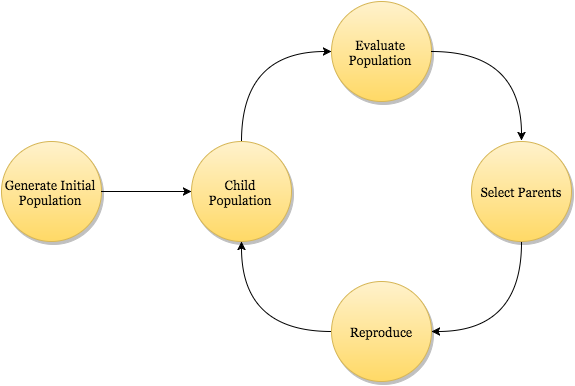
\includegraphics[scale=0.5]{GA}
%\caption{The main operations of and genetic algorithm}
%\end{center}
%\label{GA Flow chart}
%\end{figure}
%
%
%% Representation
%%\subsubsection{Representation of individuals and Reproduction}
%%The individuals (solutions) that the GA perform operations on are represented as bit-strings. Initially each bit-string is generated by randomly assigning either zero or one to each of the ''genes'' of the individual. An example of an individual is given below:
%%
%%
%%\begin{figure}[h!]
%%    \centering
%%    \begin{subfigure}[b]{0.3\textwidth}
%%        \includegraphics[width=\textwidth]{"Single Point Crossover"}
%%        \caption{Single-point crossover.}
%%        \label{fig:gull}
%%    \end{subfigure}
%%    ~ %add desired spacing between images, e. g. ~, \quad, \qquad, \hfill etc. 
%%      %(or a blank line to force the subfigure onto a new line)
%%    \begin{subfigure}[b]{0.3\textwidth}
%%        \includegraphics[width=\textwidth]{"Double Point Crossover"}
%%        \caption{Double-point crossover.}
%%        \label{fig:tiger}
%%    \end{subfigure}
%%    \caption{Crossover operations. (a) Singe point crossover at position four. (b) Double-point crossover at positions three and nine.}\label{fig:animals}
%%\end{figure}
%
%
%\subsection{The Island Model}
%The island model is an extension of the general GA where the initial population of size $N_{total}$ is partitioned into $N_{island}$ such that each island holds a population of size $N_{total} / N_{island}$. The separated populations can then evolve on each island, exploring different solutions, until a migration takes place. A migration is when some individuals from one island migrate to another island. Figure \ref{Island Model} shows an island model consisting of four island where the arrows shows legal migration routes. The topology of the island network and migration routes can take many different forms. 
%
%The advantage of using the island model, as compared to the classical GA is that in the classical GA the population can converge to a non-optimal solution quite fast, because a few individuals can take over the entire population and guide it towards a sub-optimal solution. Using the island model the probability of converging to a sub-optimal solution will decrease because each island can investigate a different part of the solution space. 
%
%
%\begin{figure}[h!]
%\begin{center}
%\includegraphics[scale=0.5]{"Island Model"}
%\caption{Island Model}
%\end{center}
%\label{Island Model}
%\end{figure}
%
%
%\subsection{The Cellular Model}
%
%
%\begin{figure}[h!]
%\begin{center}
%\includegraphics[scale=0.5]{"Cellular Model"}
%\caption{Cellular Model}
%\end{center}
%\label{Cellular Model}
%\end{figure}


\end{document}